\chapter*{Preface}\label{chapter:preface}
% c.f. https://tex.stackexchange.com/a/222961/152544
\addcontentsline{toc}{chapter}{\protect\numberline{}Preface}

The following is a summary of useful concepts in high energy particle physics.

\section{Units}\label{section:units}

\subsection{Natural Units}\label{subsection:natural_units}

The nature of high energy physics is to give descriptions of the phenomena and interactions that occur at energies that result in speeds that are close to the speed of light over very short time and distance scales.
Given this, it becomes readily apparent that the International System of Units (SI) of measurement is somewhat cumbersome to use in calculations, and a much more useful system of units would be consistent with the scale of the phenomena.
When measuring the speed of a relativistic particle it is more convenient to compare to the speed of light $\left(\text{such that }c=1\right)$ then to the number of meters per second.
Similarly, when measuring the momentum of a particle it is generally more useful to know the amount of its energy in the form of momentum compared to the amount in the form of its mass, resulting in expressing momentum in terms of energy.
This system of units is called ``Natural Units,'' and builds its measurements in terms of speed, angular momentum, and energy.
It is used extensively (if not almost exclusively) throughout high energy physics.
Quantities encountered routinely in high energy physics are given in Natural Units in \Cref{table:natural_units}.
\clearpage

\begin{table}[htpb]
 \centering
 \caption{Common quantities in particle physics given in both natural units and SI units.}
 \begin{tabular}{@{}llll@{}} \toprule
  Quantity         & Natural Units                 & Natural Units (dimensionful)            & SI Units                                              \\ \midrule
  Speed            & $1$                           & $c$                                     & $3.0\times 10^{8}~\mathrm{m}/\mathrm{s}$              \\
  Angular Momentum & $1$                           & $\hbar$                                 & $10^{34}~\mathrm{m}^2 \,\mathrm{kg}/\mathrm{s}$       \\
  Energy           & $\mathrm{GeV}$                & $\mathrm{GeV}$                          & $1.6\times 10^{-10}~\mathrm{J}$                       \\
  Momentum         & $\mathrm{GeV}$                & $\mathrm{GeV}/c$                        & $1\times 10^{-19}~\mathrm{kg}\,\mathrm{m}/\mathrm{s}$ \\
  Mass             & $\mathrm{GeV}$                & $\mathrm{GeV}/c^{2}$                    & $1.8\times 10^{-27}~\mathrm{kg}$                      \\
  Time             & $1/\mathrm{GeV}$              & $\hbar/\mathrm{GeV}$                    & $6.6\time 10^{-25}~\mathrm{s}$                        \\
  Length           & $1/\mathrm{GeV}$              & $\hbar c/\mathrm{GeV}$                  & $2\times 10^{-16}~\mathrm{m}$                         \\
  Electric Charge  & $1$                           & $e/\sqrt{4\pi \alpha_{\mathrm{em}}}$    & $5.3\times 10^{-19}~\mathrm{C}$                       \\
  Magnetic Field   & $\left(\mathrm{GeV}\right)^2$ & $\left(\mathrm{GeV}\right)^2/\hbar c^2$ & $5\times 10^{16}~\mathrm{T}$                          \\
  \bottomrule
 \end{tabular}\label{table:natural_units}%
\end{table}

\subsection{Units of Cross Section}\label{subsection:cross_section}

The ``cross section'' is the effective cross-sectional area of the event space for an given interaction to occur, and so has units of area.
It is commonly used though in the context of the fraction of the total event space that a particular process contributes (the dimensionful event space solid angle), and so is not a reflection of the physical size of an interaction.
For example, in high energy physics cross section can describe the production of a particle through a particular process, such as Higgs production through gluon-gluon fusion.
A particularly clear analogy for cross section\footnote{Made known to me by Stephen Sekula.} comes from theoretical physicist Rudolf Peierls~\cite{rhodes2012making}:
\begin{quote}
 For example, if I throw a ball at a glass window one square foot in area, there may be one chance in ten that the window will break, and nine chances in ten that the ball will just bounce.
 In the physicists' language, this particular window, for a ball thrown in this particular way, has a ``disintegration [inelastic] cross-section'' of $1/10$ square foot and an ``elastic cross-section'' of $9/10$ square foot.
\end{quote}
For the cross sections that are common in particle physics the units of ``barns'' is generally more convenient to work in, as further discussed in \Cref{subsection:luminosity_units}.
A barn is defined as
\begin{equation}
 1~\textrm{barn} = 10^{-28}~\textrm{m}^2 = 10^{-24}~\textrm{cm}^2,
 \label{eq:barn_to_area}
\end{equation}
which is roughly the cross sectional area of a uranium nucleus~\cite{web:history_physics_purdue,history:etymology_barn}.

\subsection{Units of Luminosity}\label{subsection:luminosity_units}

Tightly related to cross section is a crucial quantity of interest in high energy physics: the luminosity (both instantaneous and integrated) delivered by the particle accelerator.
The instantaneous luminosity, $\mathscr{L}$, can be defined as the number of particles incident per unit area per unit time (generally taken to be seconds),
\begin{equation}
 \mathscr{L} = \frac{\text{number of particles}}{\text{unit area} \cdot \text{second}}.
 \label{eq:instantaneous_luminosity}
\end{equation}
In accelerator physics, the unit area is generally chosen to be $\textrm{cm}^2$, giving instantaneous luminosities units of $\textrm{cm}^{-2} \cdot \textrm{s}^{-1}$,
\[
 \left[\mathscr{L}\right] = \textrm{cm}^{-2} \cdot \textrm{s}^{-1}.
\]
However, experimental particle physicists prefer to use units of inverse barns (per second) for (instantaneous) luminosities.

The context in which luminosity appears as being useful is in the form of an equation like
\begin{equation}
 N_{\textrm{events}} = \sigma_{\textrm{process}} \cdot \int \mathscr{L}\,dt
 \label{eq:events_from_luminosity}
\end{equation}
where:
\begin{itemize}
 \item $N_{\text{events}}$ is the number of events of a particular process that will be produced at the collider.
       This is what ends up exiting the collision process.
 \item $\sigma_{\textrm{process}}$ is the cross section of the particular process to occur per interaction of colliding particles.
       At the \gls{LHC} this would be the cross section per proton-proton interaction.
       This is a function of the fundamental physics that is available at the energy ranges being probed, and so is also a function of the collider's center of mass energy, $\sqrt{s}$.
       When written in an equation as such it is assumed that the cross section is also including the relevant branching ratios for the final state particles.
       That is, ${\sigma\left(pp \to H \to b\bar{b}\,\right) = \sigma\left(pp \to H\right) \cdot \mathcal{BR}\left(H \to b\bar{b}\,\right)}$.
 \item $L \equiv \int \mathscr{L}\,dt$ is the total luminosity integrated over time (the integrated luminosity)~\cite{Herr:941318}.
       This is what is delivered by the particle accelerator.
\end{itemize}

\begin{table}[htpb]
 \centering
 \caption{Instantaneous luminosities at the LHC.}
 \begin{tabular}{@{}ll@{}} \toprule
  Description                                                    & Units of $\textrm{cm}^{-2}\cdot\textrm{s}^{-1}$ \\ \midrule
  LHC Design Luminosity~\cite{Bruning:782076}                    & $10^{34}$                                       \\
  2017 ATLAS Trigger Menu Maximum~\cite{TWiki:MenuEvolution2017} & $2.0 \times 10^{34}$                            \\
  2017 Plan~\cite{Indico:MenuCoordination_2017Lumi}              & $1.7 \times 10^{34}$                            \\
  2017 Peak~\cite{TWiki:2017ATLASPeakLumi}                       & $2.09 \times 10^{34}$                           \\
  2018 Peak~\cite{TWiki:2018ATLASPeakLumi}                       & $2.1 \times 10^{34}$                            \\
  \bottomrule
 \end{tabular}\label{table:LHC_Luminosity_Goals}%
\end{table}

\begin{table}[htpb]
 \centering
 \caption{Integrated luminosity measurements in $\text{barns}^{-1}$.}
 \begin{tabular}{@{}lll@{}} \toprule
  Units                & Units of $\textrm{cm}^{-2}$ & Units of $\textrm{fb}^{-1}$ \\ \midrule
  $\textrm{barn}^{-1}$ & $10^{24}$                   & $10^{-15}$                  \\
  $\textrm{mb}^{-1}$   & $10^{27}$                   & $10^{-12}$                  \\
  $\mu\textrm{b}^{-1}$ & $10^{30}$                   & $10^{-9}$                   \\
  $\textrm{nb}^{-1}$   & $10^{33}$                   & $10^{-6}$                   \\
  $\textrm{pb}^{-1}$   & $10^{36}$                   & $10^{-3}$                   \\
  $\textrm{fb}^{-1}$   & $10^{39}$                   & $10^{0}$                    \\
  $\textrm{ab}^{-1}$   & $10^{42}$                   & $10^{3}$                    \\
  \bottomrule
 \end{tabular}\label{table:Luminosity}%
\end{table}

\clearpage
\section{Coordinates}\label{section:coordinates}

The LHC coordinate system, seen in \Cref{fig:LHC_coordinate_system}, is a rectangular coordinate system defined relative to the LHC ring and the LHC beamline.
At any point, the positive $x$ direction is defined as the direction that points radially inward to the center of the LHC ring.
The positive $y$ direction is then defined as pointing upwards --- radially outward from the center of the Earth --- leaving the positive $z$ direction pointing along the beamline.

\begin{figure}[htbp]
 \centering
 \includegraphics[width=0.8\linewidth]{preface/LHC_coordinate_system.pdf}
 \caption{The LHC coordinate system as seen from the ATLAS detector.}
 \label{fig:LHC_coordinate_system}
\end{figure}

While the LHC coordinate system is Cartesian, the preferred coordinate system for describing LHC events is not.
As the ATLAS detector is arranged cylindrically around the beamline of the LHC --- such that most of its detector components are transverse to the beamline --- the coordinate system that is used to describe events in ATLAS is characterized by a particle's transverse momentum, pseudorapidity, and azimuthal angle: $\left(p_T, \eta, \phi\right)$.
The polar angle, $\theta$, is defined as the angle relative to the beam axis, and the azimuthal angle, $\phi$, is measured around the beam axis.

\Gls{Pseudorapidity} is then defined as
\begin{equation}
 \eta = - \ln \left(\tan \frac{\theta}{2}\right)
 \label{eq:pseudorapidity}
\end{equation}
to be a good approximation in the high energy regime of the \gls{rapidity} of a particle --- a measurement of the velocity of a particle longitudinal to the beam axis,
\begin{equation}
 y = \frac{1}{2} \ln \left(\frac{E + p_{z}}{E - p_{z}}\right).
 \label{eq:rapidity}
\end{equation}
As the beam axis is defined as $\hat{\vec{z}}$, such that $p_{z} = \abs{\vec{p}} \cos\theta$, then it is seen that in the relativistic limit, $\abs{\vec{p}} \gg m$, the rapidity reduces to the pseudorapidity
\[
 \begin{split}
  y\left(\abs{\vec{p}} \gg m\right)   &\approx \frac{1}{2} \ln \left(\frac{p + p\cos\theta}{p - p\cos\theta}\right)\\
  &\approx \frac{1}{2} \ln \left(\frac{2 \cos^{2} \frac{\theta}{2}}{2 \sin^{2} \frac{\theta}{2}}\right) \\
  &\approx - \ln \left(\tan \frac{\theta}{2}\right) = \eta.
 \end{split}
\]
It is clear that the rapidity and the pseudorapidity are not \Glspl{Lorentz invariant}.
However, for a Lorentz \gls{boost} --- a Lorentz transformation without any rotations --- of speed $\beta$ along the beam axis, $\hat{\vec{z}}$,
\[
 \begin{pmatrix}
  E' \\
  p_{z}'
 \end{pmatrix}
 =
 \begin{pmatrix}%
  \gamma       & -\gamma\beta \\%
  -\gamma\beta & \gamma
 \end{pmatrix}%
 \begin{pmatrix}
  E \\
  p_{z}
 \end{pmatrix}\,,
\]
it is seen\footnote{Glossing over some algebra and hyperbolic trigonometric identities.} that the rapidity for a particle under the boost is the sum of the original rapidity and a constant of the boost
\[
 \begin{split}
  y'  &= \frac{1}{2} \ln \left(\frac{E' + p_{z}'}{E' - p_{z}'}\right) \\
  &= \frac{1}{2} \ln \left(\frac{E - \beta p_{z} + p_{z} - \beta E}{E - \beta p_{z} - p_{z} + \beta E}\right) \\
  &= \frac{1}{2} \ln \left(\frac{E + p_{z}}{E - p_{z}}\right) + \frac{1}{2} \ln \left(\frac{1 - \beta}{1 + \beta}\right) \\
  &= y - \tanh^{-1}\beta\,.
 \end{split}
\]
Thus, the \emph{difference in rapidities} between two particles is seen to be independent of the boost and so is a \Gls{Lorentz invariant}.
Defining the distance metric\footnote{$\Delta R$ is an angular distance in $\left(\eta, \phi\right)$ space, and can be thought of as a solid angle.} for two particles in $\left(\eta, \phi\right)$ space as
\begin{equation}
 \Delta R = \sqrt{\left(\Delta\eta\right)^{2} + \left(\Delta\phi\right)^{2}}
 \label{eq:DeltaR}
\end{equation}
it is seen that $\Delta R$ is by construction invariant to boosts along the beam axis.
As a result, \emph{translations} in $\eta$ of particles correspond to \glspl{boost} of the particles along the beamline.

For experiments at high energy colliders, the pseudorapidity offers a distinct advantage in the high energy limit as it only requires angular information while giving an excellent approximation to the rapidity.
Measuring both the energy and the full momentum for highly relativistic particles can be quite difficult, and as the differences between the rapidity and the pseudorapidity can quickly become very small, pseudorapidity is the favored measurement for experimental results.
Values of the pseudorapidity for values of the polar angle are summarized in \Cref{table:pseudorapidity_angles} and are plotted along with the form of \Cref{eq:rapidity} in \Cref{fig:pseudorapidity_angles}.

\begin{table}[htpb]
 \centering
 \caption{Polar angles relative to the LHC beam axis, $\theta$, and their corresponding pseudorapiditities, $\eta$.}
 \begin{tabular}{@{}cr@{}} \toprule
  Polar angle $(\theta)$ & Pseudorapidity $(\eta)$ \\ \midrule
  $\frac{\pi}{2}$        & $0$                     \\
  $\frac{\pi}{4}$        & $0.88137$               \\
  $\frac{\pi}{8}$        & $1.61489$               \\
  $\frac{\pi}{16}$       & $2.31779$               \\
  $\frac{\pi}{32}$       & $3.01335$               \\
  \bottomrule
 \end{tabular}\label{table:pseudorapidity_angles}%
\end{table}

\begin{figure}[htbp]
 \centering
 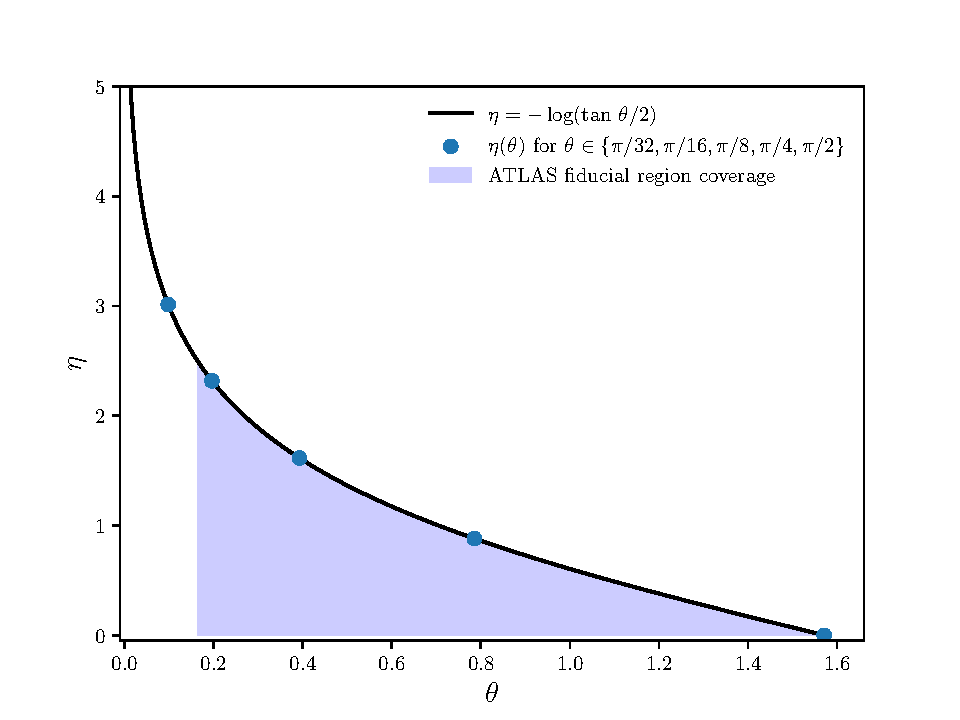
\includegraphics[width=0.8\linewidth]{preface/pseudorapidity.pdf}
 \caption[Pseudorapidity as a function of the polar angle.]{%
  Pseudorapidity, $\eta = - \ln \left(\tan \frac{\theta}{2}\right)$, as a function of the polar angle, $\theta$.
  The example markers are the points given in \Cref{table:pseudorapidity_angles}.
  The blue shaded region indicates the polar angle coverage up to $\eta = 2.5$, which is the end of the fiducial region coverage by the ATLAS inner detector tracking.}
 \label{fig:pseudorapidity_angles}
\end{figure}

\clearpage
\section{Statistics}\label{section:statistics}

Statistics in particle physics

\subsection{Intervals and limits}\label{section:intervals_and_limits}

In addition to point estimates that determine an estimator, $\hat{\theta}$, of a parameter $\theta$, interval estimates give statistical precision to the measured value.
A common example of such an interval estimate is the set of points bounded by the point estimate and the estimated standard deviation: $\left[\hat{\theta} - \sigma_{\hat{\theta}}, \hat{\theta} + \sigma_{\hat{\theta}}\right]$.
The following is a short discussion of the construction, interpretation, and use of these intervals in the frequentist and Bayesian paradigms.

\subsubsection{Frequentist Confidence Intervals}

In the frequentist paradigm, a $1-\alpha$ confidence level (CL) confidence interval (CI) is an interval estimate that covers the true value of the parameter, $\theta$, $1-\alpha$ of the time it is constructed.
So the $95\%$ confidence level confidence interval covers the true value $95\%$ of the time it is constructed.
The method for constructing confidence intervals is called the ``Neyman Construction''~\cite{Neyman:1937uhy}, and results from inverting hypothesis tests.
This confidence interval construction can be described as a random variable that is the set of parameter points, $\left\{\vec{\theta}\right\}$, where the null hypothesis of each parameter point $\theta$ is accepted, $p\left(t > k_{\alpha}\middle| \theta\right) < \alpha$,

\begin{equation}
 \mathrm{CI}_{1-\alpha} = \left\{\vec{\theta}\,\middle| \,p\left(t > k_{\alpha}\middle| \vec{\theta}\right) < \alpha\right\}\,.
 \label{eq:confidence_interval}
\end{equation}

By construction, a hypothesis test of size $\alpha$ should accept the null hypothesis, given that the null is true, $(1-\alpha)$ of the time~\cite{Cranmer:2015nia}.\\

It is very important to take care in interpreting the meaning of the confidence interval, as it is often misunderstood and misused in analysis.
The confidence interval is constructed from the observed data%
\footnote{The data are a random variable in the frequentist paradigm.}
and so is a random variable and reflects information regarding the constructed estimator --- not the true parameter.
The confidence interval does \emph{not} give the interval in which there is a $1-\alpha$ probability of finding the true parameter value.
This is manifestly Bayesian and in fact is the interpretation of a Bayesian credible interval.
Keeping the definition of frequentist probability tightly in mind, the confidence interval should be interpreted as an interval of parameter values that $1-\alpha$ \emph{of the times is is constructed} contains the true parameter value.
Given this, in the frequentist paradigm one is \emph{unable} to make any statement on the probability that the true parameter value is contained in any specific confidence interval beyond the tautology that the true parameter is either contained in the it or it is not.
Any misuse of this result is not from a failing of the paradigm, but a misplaced desire of the analyst to have different questions answered than were asked.\\

In terms of computing a confidence interval, from observations that are governed by $\theta$ a test statistic, $t$, that is an estimator of $\theta$ is constructed.
For each value of the parameter to be tested, there exists an interval $\left[t_{1}, t_{2}\right]$ such that the probability of $t \in \left[t_{1}, t_{2}\right]$ is
\begin{equation}
 p\left(t_{1} < t < t_{2}\middle|\theta\right) = \int\limits_{t_{1}}^{t_{2}} f\left(t\middle|\,\theta\right)\,dt = 1-\alpha\,.
 \label{eq:confidence_interval_coverage}
\end{equation}
This interval represents a constant line segment in the $\left(t, \theta\right)$ parameter space plane at the given value of $\theta$.
By repeating this procedure for every value of $\theta$ to be tested, a band of line segments --- a ``confidence belt'' --- is created that is bound between the curves $\theta\left(t_{1}\right)$ and $\theta\left(t_{2}\right)$, as shown in the example in \Cref{fig:confidence_belt}.
Then, for any given observed value of the test statistic, $t'$, a boundary at $t = t'$ can be drawn in the plane that intersects the confidence belt at the points $\left(t', \theta_{2}\right)$ and $\left(t', \theta_{1}\right)$.
This resulting range of parameter values $\left[\theta_{1}, \theta_{2}\right]$ is the confidence interval~\cite{Cranmer:2015nia,PDG2018:Ch39}.\\

\begin{figure}[htbp]
 \centering
 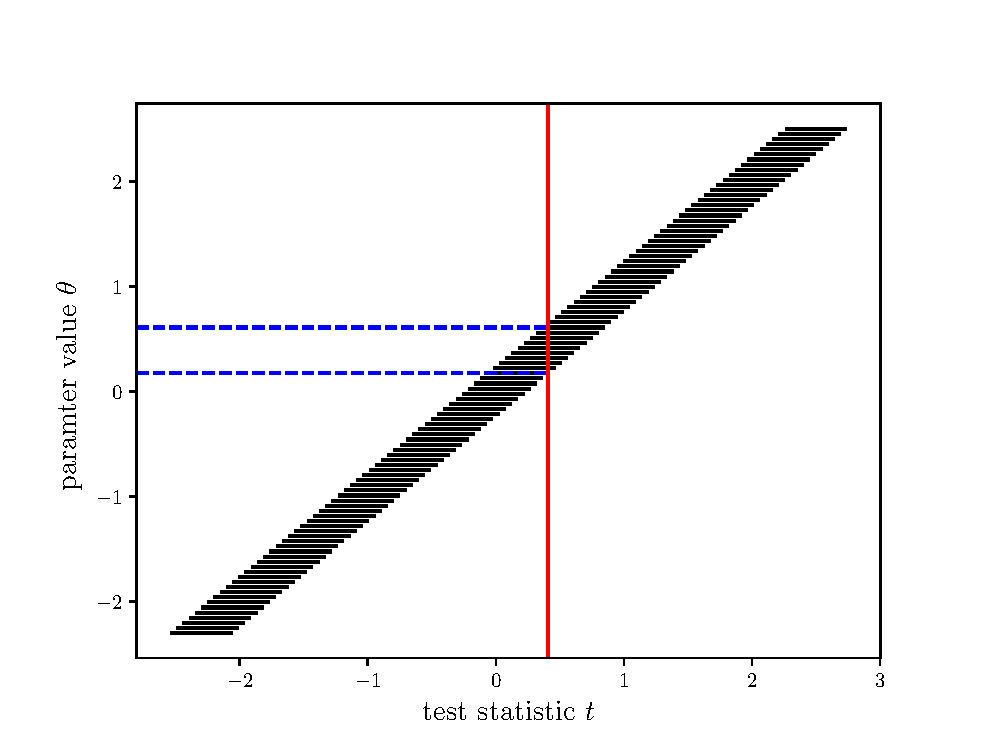
\includegraphics[width=0.4\linewidth]{preface/confidence_belt.eps}
 \caption{Example sketch of the construction of a confidence belt showing an observation in red intersecting the belt and the corresponding confidence interval as the parameter values bounded between the two blue dashed lines.}\label{fig:confidence_belt}
\end{figure}

The conditions of coverage from \Cref{eq:confidence_interval_coverage} do not uniquely specify $t_{1}$ and $t_{2}$, which allows for analysis specific choices to be made.
If central intervals are chosen, then the probabilities excluded below $t_{1}$ and $t_{2}$ are both $\alpha/2$.
In the event that only an upper (or lower) limit is of interest, as is common in searches for new physics where no excess has been observed, then the probability excluded below $t_{1}$ (or above $t_{2}$) is zero.
Alternatively, if the test statistic used is based on the likelihood ratio
\[
 \lambda = \frac{L\left(\theta\middle|\, t\right)}{L(\hat{\theta}|\, t)},
\]
the test statistic can be profiled to determine the range $\left[t_{1}, t_{2}\right]$.
Using such a test statistic results in the Feldman-Cousins confidence intervals~\cite{Feldman:1997qc}.\\

As the confidence interval can be a difficult concept to describe, a simple illustrative example follows.
Consider $n$ observations $\vec{x} = \left\{x_{1}, \cdots, x_{n}\right\}$ that are drawn from a Normal distribution with unknown mean $\theta$ and width $\sigma_{\theta}$.
This results in a sample mean $\hat{\theta}$ and standard deviation $\sigma_{\hat{\theta}}$.
To construct a $95\%$ confidence level central confidence interval for $\theta$, the test statistic $t = \left(\hat{\theta} - \theta\right)/\sigma_{\hat{\theta}}$ can be used such that ${p\left(t_{1} < t < t_{2}\middle|\theta\right) = 0.95}$, where $t_{1}$ and $t_{2}$ are respectively the $2.5$th percentile and $97.5$th percentile%
\footnote{$t_{1} = \mathrm{CDF}^{-1}\left(\alpha/2\right)$ and $t_{2} = \mathrm{CDF}^{-1}\left(1 - \alpha/2\right)$.}
of the Student's $t$-distribution for $n-1$ degrees of freedom, mean $\mu=\hat{\theta}$ and standard deviation $\sigma=\sigma_{\hat{\theta}}$.
Transforming the Student's $t$-distribution by $t' = \left(t-\hat{\theta}\right)/\sigma_{\hat{\theta}}$ to have $\mu=0, \sigma=1$ simplifies to ${p\left(-d < t' < d\middle|\theta\right) = 0.95}$.
Transforming to parameter space, ${p\left(\hat{\theta} - d\, \sigma_{\hat{\theta}} < \theta < \hat{\theta} + d\, \sigma_{\hat{\theta}}\right)  = 0.95}$, this gives a confidence interval of $\left[\hat{\theta} - d\, \sigma_{\hat{\theta}}, \hat{\theta} + d\, \sigma_{\hat{\theta}}\right]$.
Confidence intervals following this example construction are simulated and shown in \Cref{fig:confidence_intervals}.

\begin{figure}[htbp]
 \centering
 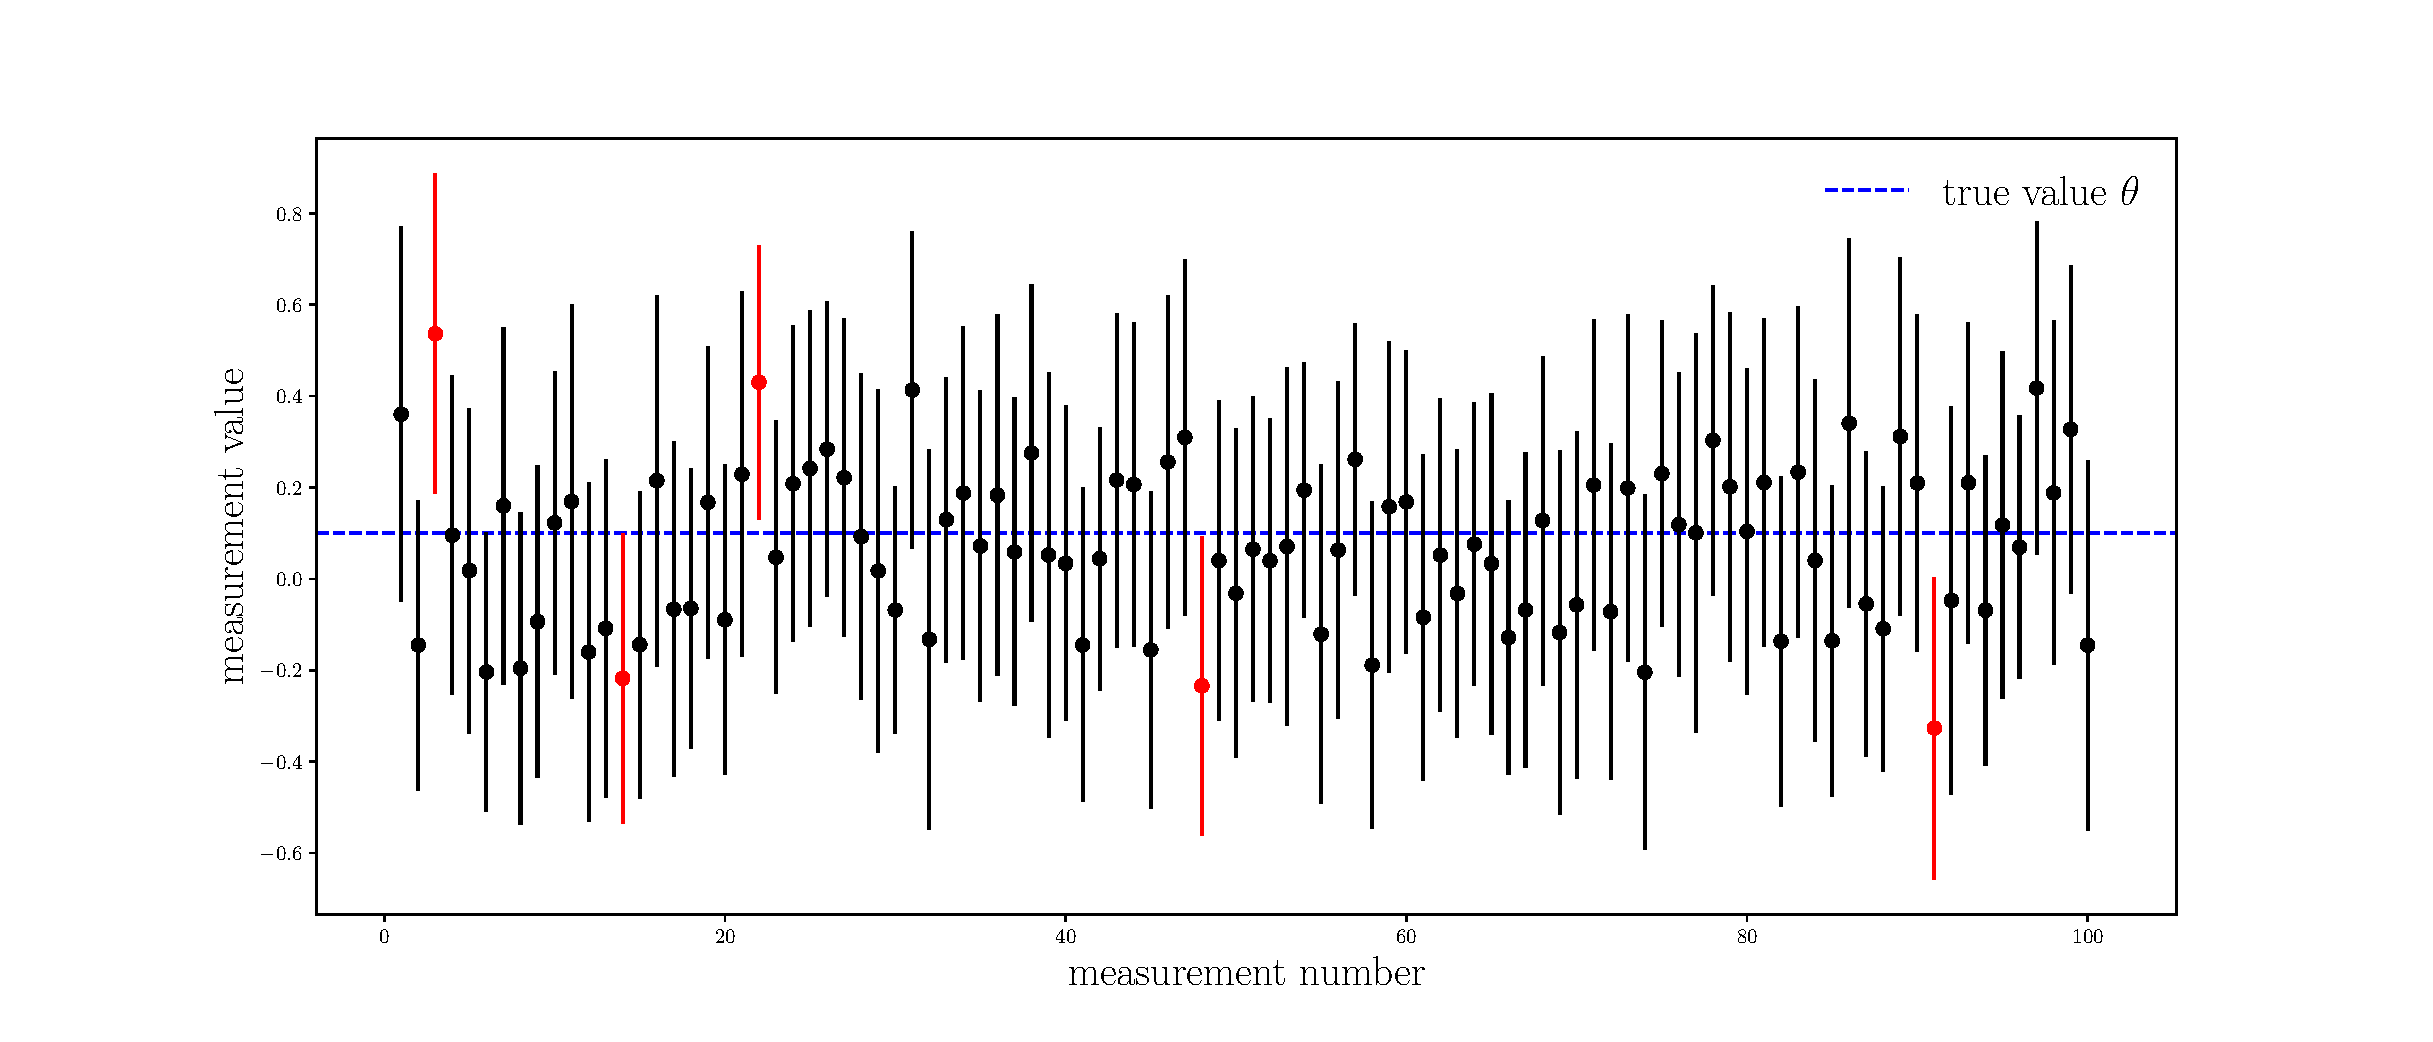
\includegraphics[width=\linewidth]{preface/confidence_intervals.eps}
 \caption{An example of 100 point estimates and associated $95\%$ confidence level confidence intervals of parameter value $\theta$.
  Confidence intervals that do not include the true value $\theta$ (dashed blue line) are colored red.}
 \label{fig:confidence_intervals}
\end{figure}

\subsubsection{Bayesian Credible Intervals}

In the Bayesian paradigm, a $1-\alpha$ credibility level (CL) credible interval (CI)%
\footnote{CL and CI are used for abbreviations for both the frequentist and Bayesian intervals.
 It will be made clear to the reader from context which paradigm is being considered.}
is an interval estimate where there is a $1-\alpha$ probability of containing the true parameter value --- which is a random variable.
As a result, it is simply the interval of the posterior predictive distribution $\left[\theta_{1}, \theta_{2}\right]$ that when integrated over gives a probability of $1-\alpha$,

\begin{equation}
 p\left(\theta_{1} < \theta < \theta_{2}\middle|\vec{x}\right) = \int\limits_{\theta_{1}}^{\theta_{2}} p\left(\theta\middle|\,\vec{x}\right)\,d\theta = 1-\alpha\,.
 \label{eq:credible_interval_coverage}
\end{equation}

As in the frequentist paradigm, there are different ways to select the credible interval range.
One can choose the shortest interval,%
\footnote{For a unimodal distribution this interval is known as the highest posterior density interval (HPD).}
the interval where probabilities excluded below $\theta_{1}$ and above $\theta_{2}$ are both $\alpha/2$ (this interval includes the median), the interval centered at the mean of the posterior (if the mean exists), or the intervals corresponding to upper (or lower) limits which reduce \Cref{eq:credible_interval_coverage} to the CDF (or CCDF) of $\theta$.\\

As a final word on interval estimates, it is worth remembering that the frequentist and Bayesian paradigms address different questions and so make different statements with their intervals.
\begin{itemize}
 \item Frequentist: When a confidence interval is constructed on future data, the constructed interval will contain the true parameter value with a probability (frequency) of $1-\alpha$.
 \item Bayesian: Given the observed data, there is a $1-\alpha$ probability that the true parameter value is contained by the constructed credible interval.
\end{itemize}


\section{Open Source Tools}\label{section:open_source}

This thesis and the researched described in it were made possible only through use of open source software.
The analysis was written in the open source languages \texttt{C++} and \texttt{Python} and made extensive use of the \texttt{ROOT} data analysis framework.
Similarly, parts of the analysis were conducted in Python and leveraged the SciPy ecosystem, most notably the NumPy and matplotlib libraries.
Additionally, the Keras library was used to interface with the TensorFlow machine learning framework for parts of the analysis.
The thesis itself was written in \LaTeXe, built using \texttt{latexmk} and \texttt{Make}, and versioned with Git.
Scientific research is built upon the open source community and tools, and this work would not have been made possible without it.
